\chapter{Data preprocessing}
\label{sec:data_preprocessing}

\section{Preprocessing Rationale and Technical Constraints}
\label{sec:preprocessing_rationale}
DNA methylation arrays provide high-dimensional, genome-wide measurements 
in which biological variability and platform-specific technical artefacts 
are inevitably superimposed. The exploratory analyses of Chapter~\ref{sec:data_preparation_exploration} 
revealed a consistent picture across all three cohorts: Normal and Adjacent 
tissues exhibit nearly identical global methylation distributions, 
overlapping variance profiles, and indistinguishable sample-level 
correlation structure. Meaningful differences between tissue states emerge 
exclusively at focal CpG loci—as quantified by locus-specific $\Delta\beta$ 
distributions and outlier burden ratios—and remain subtle even at that 
scale (mean $|\Delta\beta|$ ranging from 0.009 in GSE69914 to 0.031 in 
GSE287331). This characteristic makes the Normal--Adjacent signal 
particularly vulnerable to technical confounders, which operate at a 
comparable or larger scale than the biological effect of interest. 
Preprocessing must therefore be precise: aggressive enough to remove 
technical noise, but conservative enough to preserve the subtle epigenetic 
drift that motivates this thesis.

Three main classes of technical issues must be systematically addressed 
before any statistical modelling can proceed. First, \textbf{probe-design 
bias} intrinsic to the Infinium platform arises from the coexistence of 
two chemically distinct probe types (Type~I and Type~II), which produce 
inherently different $\beta$-value distributions and can distort 
cross-sample comparability if not corrected~\cite{Triche2013, Fortin2017}. 
This issue is not uniform across datasets: as will be shown in 
Section~\ref{sec:dataset_specific}, GSE69914 and GSE225845 were released 
with normalization already applied by the original authors, whereas 
GSE287331 shows clear diagnostic evidence of missing probe-type correction, 
requiring an additional preprocessing decision with non-trivial consequences 
for downstream group separation. Second, a subset of \textbf{unreliable 
or biologically confounded probes}---including cross-reactive loci, 
SNP-affected sites, non-CpG targets, and sex-chromosome probes---introduces 
systematic measurement error that can generate spurious associations or 
mask genuine methylation differences~\cite{WilhelmBenartzi2013, Xu2021}. 
Third, the \textbf{statistical scale of $\beta$-values} poses inferential 
challenges: the bounded $[0,1]$ support and strong mean-dependent 
heteroscedasticity of $\beta$-values violate the assumptions of standard 
parametric models, motivating transformation to a more statistically 
well-behaved representation prior to modelling~\cite{Triche2013}.

This chapter addresses these three issues through a structured, 
platform-aware preprocessing pipeline applied consistently across all 
cohorts. Section~\ref{sec:pipeline} describes the general framework and 
the rationale for each step. Section~\ref{sec:dataset_specific} documents 
the dataset-specific application, focusing on the decisions that deviate 
from the standard workflow---most notably the handling of probe-type bias 
in GSE287331, where the tension between technical correction and 
preservation of biological structure requires explicit justification. 
Section~\ref{sec:inter_preprocessing} summarises the effect of 
preprocessing on CpG dimensionality and cross-dataset overlap, providing 
the basis for the feature selection strategy developed in Chapter~\ref{sec:feature_selection}.

\section{General Preprocessing Framework}
\label{sec:pipeline}

This section describes the general preprocessing framework applied to all 
three methylation datasets. The pipeline comprises four sequential steps, 
each addressing a distinct class of technical issue identified in the 
overview above. Two of these steps—data integrity verification and 
Infinium probe-design bias correction—require dataset-specific decisions 
whose rationale and consequences are discussed in 
Section~\ref{sec:dataset_specific}. The remaining two steps—technical 
probe filtering and $\beta$-to-$M$ transformation—are applied uniformly 
across all cohorts following the same protocol.

%------------------------------------------------------------------
\subsection{Structural Integrity and Cohort Harmonization}
\label{subsec:step0}
%------------------------------------------------------------------

Prior to any preprocessing operation, each dataset undergoes a structural 
verification stage to ensure the consistency and completeness of the input 
data. This step checks for correct alignment between the methylation matrix 
and its associated phenotype table, verifies sample identifier uniqueness, 
and confirms the absence of missing metadata fields. Only samples for which 
both a complete methylation profile and a valid tissue label are available 
are retained for downstream analysis.

Probe-level and sample-level missingness in the $\beta$-value matrix is 
also assessed at this stage. For two of the three datasets (GSE69914 and 
GSE225845), the released matrices are fully observed and require no 
imputation. For GSE287331, a non-negligible fraction of CpG sites exhibits 
missing values across samples, necessitating a dedicated filtering and 
imputation strategy consistent with current recommendations for 
EPIC-array quality control~\cite{islam2019_pediatric_dnamm, mansell2019guidance}. The 
dataset-specific treatment of missingness is detailed in 
Section~\ref{subsec:gse287331_data_prep}.

Finally, cohort harmonization is applied where necessary to align tissue 
labels to the three-class framework (Normal, Adjacent, Tumor) adopted 
uniformly across datasets. Samples belonging to tissue categories outside 
this framework are excluded at this stage to ensure cross-dataset 
comparability.

%------------------------------------------------------------------
\subsection{Probe-Type Bias Diagnostics and Correction}
\label{subsec:step1}
%------------------------------------------------------------------

A well-documented source of systematic bias in Illumina Infinium 
methylation arrays is the coexistence of two chemically distinct probe 
designs. Type~I probes use two bead types per CpG (one for the methylated 
channel, one for the unmethylated channel), whereas Type~II probes use a 
single bead type and rely on single-base extension with two-color 
detection. This design difference produces inherently distinct 
$\beta$-value distributions for the two probe types: Type~I probes tend 
to yield more extreme values near 0 and 1, while Type~II probes exhibit 
a broader, intermediate distribution. If uncorrected, this imbalance 
propagates into downstream statistical analyses and can generate 
probe-type-specific artefacts in differential methylation 
testing~\cite{Teschendorff2013BMIQ, maksimovic2012}.

The canonical approach to mitigating this bias is Beta-Mixture Quantile 
normalisation (BMIQ), introduced by Teschendorff et 
al.~\cite{Teschendorff2013BMIQ}. BMIQ explicitly models probe-type bias 
at the $\beta$-value level through a state-aware distributional alignment 
procedure. For each sample independently, a three-component Beta mixture model is 
first fitted to the $\beta$-value distribution of Type~I probes, 
representing unmethylated, partially methylated, and fully methylated 
states. These fitted components define the reference state-specific 
distributions. Type~II probes are then probabilistically assigned to one 
of the three methylation states based on their $\beta$-values, and within 
each state a quantile-mapping step is applied to align the Type~II 
distribution to the corresponding Type~I reference distribution. Because the procedure is performed independently for each sample, BMIQ 
does not introduce cross-sample information or global harmonisation across 
tissue classes; it strictly corrects within-sample probe-type bias.

For each dataset, a systematic diagnostic is performed prior to any 
correction step~\cite{Teschendorff2013BMIQ, Wang2015Normalization450K}: probes are 
stratified by design type using the official Illumina manifest, and two 
complementary assessments are carried out—(i) a density comparison of 
$\beta$-value distributions for Type~I and Type~II probes, and (ii) a 
quantile--quantile plot of Type~II versus Type~I quantiles, with the 
median absolute deviation (MAD) of the empirical Q--Q curve from the identity line 
as a scalar diagnostic metric. Datasets for which the original authors 
applied BMIQ or an equivalent normalisation are expected to exhibit 
near-overlapping distributions and a MAD close to zero; datasets lacking 
probe-type correction will display a pronounced distributional mismatch 
and elevated MAD.

The outcome of this diagnostic, and the corrective action taken, differs 
across cohorts and is reported in full in Section~\ref{sec:dataset_specific}. 
Critically, the decision of whether to apply BMIQ is not made 
mechanically: as discussed in Section~\ref{subsec:gse287331_data_prep}, BMIQ 
correction can attenuate genuine biological structure when group-level 
differences are expressed as broad distributional shifts, a phenomenon 
documented in systematic evaluations of EPIC-array normalisation 
methods~\cite{Yousefi2013, Welsh2023EPICnorm, Liu2016Processing}. The choice between 
correcting and preserving the raw data is therefore made on the basis of 
empirical evidence from the diagnostic plots and quantitative assessment 
of group separability before and after correction.

%------------------------------------------------------------------
\subsection{Technical Probe Filtering}
\label{subsec:step2}
%------------------------------------------------------------------

After addressing probe-design bias, unreliable CpG loci are removed 
through a systematic filtering procedure based on curated external 
annotation resources. The objective is to exclude probes whose measured 
$\beta$-values may reflect technical measurement error rather than 
genuine DNA methylation, thereby reducing noise and improving the 
reliability of downstream differential analyses. Four categories of technically problematic probes are systematically excluded.

\paragraph{Cross-reactive and multi-mapping probes.} Probes that 
hybridise to multiple genomic loci produce $\beta$-values that cannot 
be unambiguously attributed to a single CpG site. These are identified 
using the catalogues of Naeem et al.~\cite{naeem2014}, Chen et 
al.~\cite{chen2013}, Pidsley et al.~\cite{pidsley2016}, Zhou et 
al.~\cite{zhou2017}, and McCartney et al.~\cite{mccartney2016}. Full 
descriptions of each resource are provided in Appendix~\ref{sec:probe-filters}.

\paragraph{SNP-affected probes.} Probes whose interrogated CpG 
dinucleotide, single-base extension site, or probe body overlaps a 
common genetic variant may measure genotype rather than methylation 
status, producing population-stratified artefacts in group 
comparisons~\cite{zhou2017, pidsley2016}. These are excluded using the 
\texttt{MASK\_snp5} and \texttt{MASK\_extBase} fields from the Zhou 
annotation~\cite{zhou2017}, supplemented by variant-aware lists from 
Naeem et al.~\cite{naeem2014}.

\paragraph{Non-CpG probes.} Probes targeting non-CpG cytosine contexts 
(identified by the \texttt{ch} prefix in Illumina probe identifiers) are 
excluded, as their interpretation differs from canonical CpG methylation 
and is outside the scope of this analysis~\cite{zhou2017, pidsley2016}.

\paragraph{Sex-chromosome probes.} Probes located on chromosomes X and Y 
are removed to prevent sex-driven confounding effects. Sex-chromosome 
CpGs exhibit substantially different methylation profiles between males 
and females, and including them in joint normalisation has been shown to 
introduce artificial sex-related bias into autosomal 
probes~\cite{Wang2022InterpolatedXY}. Since the datasets analysed here contain samples 
from both sexes and sex-specific methylation is not the object of 
investigation, removal therefore represents a conservative strategy to prevent confounding without compromising autosomal inference~\cite{maksimovic2012}.

The filtering resources are applied under a union criterion: a probe is removed if it appears in at least one curated list. Platform-specific 
manifests (HumanMethylation450 v1.2 for GSE69914~\cite{Illumina450kAnno}; 
MethylationEPIC v1.0 B5 for GSE225845 and GSE287331~\cite{IlluminaEPIC}) 
are used for manifest-based validation, chromosome annotation, and 
non-CpG probe identification. The number of probes flagged by each 
resource, and the redundancy of flags across resources, are reported 
per-dataset in Section~\ref{sec:dataset_specific}.

%------------------------------------------------------------------
\subsection{Statistical Transformation: $\beta$-to-$M$ Values}
\label{subsec:step3}
%------------------------------------------------------------------

The final preprocessing step transforms the filtered $\beta$-value matrix 
into $M$-values prior to statistical modelling. As defined in Equation~\eqref{eq:beta_definition}, $\beta$-values are bounded proportions in $[0,1]$ derived from methylated and unmethylated probe intensities. While $\beta$-values are intuitive and directly 
interpretable as fractional methylation, their bounded support induces 
strong mean-dependent heteroscedasticity: variance is inflated near 
intermediate values ($\beta \approx 0.5$) and compressed near the 
boundaries, violating the homoscedasticity assumptions underlying 
standard linear modelling frameworks~\cite{Du2010}.

The logit transformation to $M$-values,

\begin{equation}
    M = \log_2\!\left(\frac{\beta + \varepsilon}{1 - \beta + \varepsilon}\right),
    \quad \varepsilon = 10^{-6},
    \label{eq:mvalue}
\end{equation}

maps $\beta \in (0,1)$ to an unbounded real-valued scale and 
substantially stabilises the mean--variance relationship~\cite{Du2010}. 
As shown in their analysis, the relationship between $\beta$ and $M$-values 
is a logit transformation yielding an approximately linear correspondence 
in the intermediate methylation range and nonlinear compression at the 
extremes. The small offset $\varepsilon$ is introduced to handle boundary values 
numerically. The resulting $M$-value distributions are approximately 
symmetric and exhibit markedly flatter variance profiles across the full 
methylation range, making them the standard input for differential methylation analysis within linear modelling frameworks and related inferential procedures~\cite{Triche2013, Fortin2017, Thienpont2016}.

It is important to note that $M$-values are adopted exclusively for 
statistical modelling: $\beta$-values are retained in parallel for 
biological interpretation, effect-size quantification, and visualisation, 
following the dual-representation convention recommended by Du et 
al.~\cite{Du2010} and widely adopted in the 
literature~\cite{Thienpont2016, Reinius2012}. 

The transformation is applied to the complete post-filtering matrix for 
each dataset. Distributional diagnostics confirming the expected 
variance-stabilising effect are reported in 
Section~\ref{sec:dataset_specific}. This choice is consistent with the feature-selection and modelling procedures developed in the subsequent chapter~\ref{sec:feature_selection}, which rely on variance-based ranking, linear statistics, and stability criteria that assume approximately homoscedastic behaviour.

\section{Dataset-Specific Implementation}
\label{sec:dataset_specific}

This section documents the dataset-specific application of the preprocessing pipeline described in Section~\ref{sec:pipeline}. For each cohort, the outcome of structural verification, probe-type bias diagnostics, technical probe filtering, and $\beta$-to-$M$ transformation is reported in detail. Although the general framework is applied consistently across all datasets, certain steps—most notably probe-type bias correction and handling of missing values—require cohort-specific decisions. These are explicitly justified within each subsection.

The results are presented separately for GSE69914 (Section~\ref{subsec:gse69914_preproc}), GSE225845 (Section~\ref{subsec:gse225845_preproc}), and GSE287331 (Section~\ref{subsec:gse287331_data_prep}).


% ============================================================
\subsection{Dataset GSE69914}
\label{subsec:gse69914_preproc}
% ============================================================
\begin{figure}[t]
    \centering
    \begin{subfigure}[t]{0.48\linewidth}
        \centering
        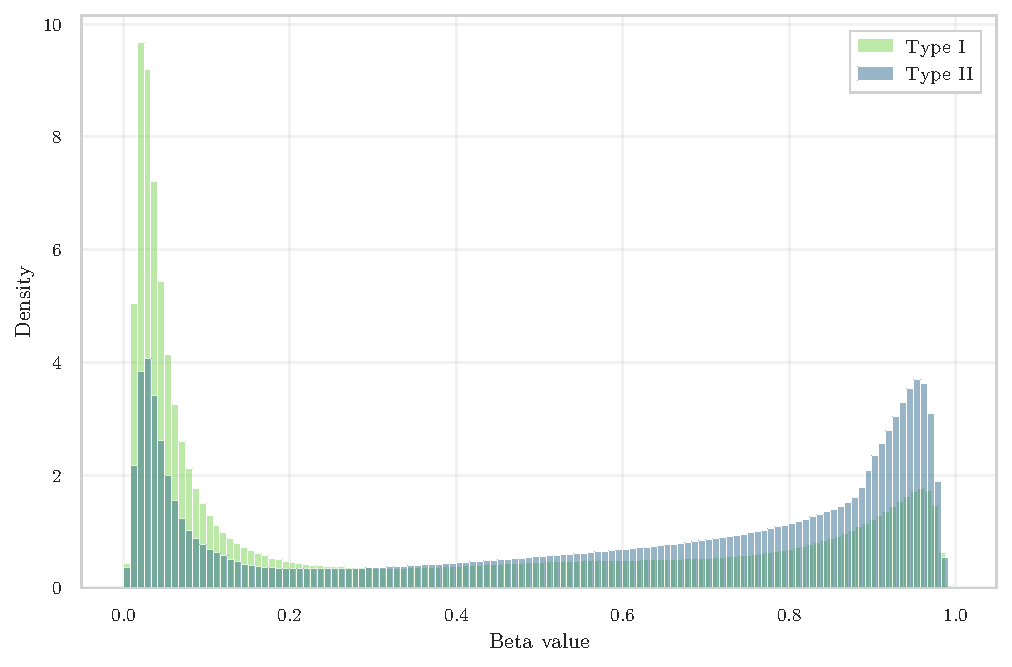
\includegraphics[height=4.5cm,keepaspectratio]{images/cap4/GSE69914_type_bias_density.pdf}
        \caption{$\beta$-value density by probe type.}
        \label{fig:type_bias_density}
    \end{subfigure}
    \hfill
    \begin{subfigure}[t]{0.48\linewidth}
        \centering
        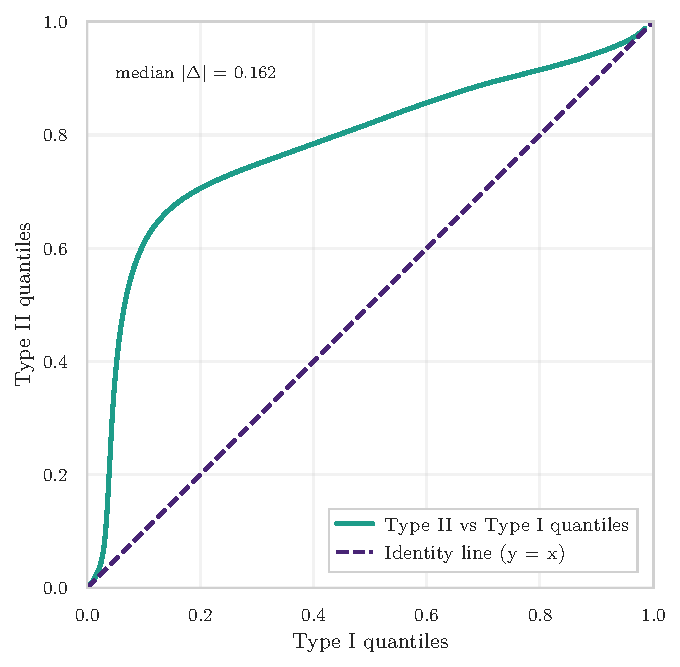
\includegraphics[height=4.5cm,keepaspectratio]{images/cap4/GSE69914_type_bias_qqplot.pdf}
        \caption{Q--Q plot (Type~II vs.~Type~I).}
        \label{fig:type_bias_qq}
    \end{subfigure}
    \caption{Infinium Type~I/II bias diagnostics in GSE69914.}
    \label{fig:type_bias_combined}
\end{figure}

\paragraph{Structural Integrity and Cohort Harmonization}
\label{par:gse69914_step0}
The dataset comprises 397 samples and 485{,}512 CpGs at load time. All sample identifiers are unique, and the phenotype table contains complete metadata for the required fields.
Alignment between the phenotype annotation and the $\beta$-value matrix is exact. The methylation matrix is fully observed, with no missing CpG values and no incomplete samples. No exclusion or imputation was required.

\paragraph{Probe-Type Bias Diagnostics and Correction}
\label{par:gse69914_typebias}

Raw intensity data were reported to have been processed by the original authors using the \texttt{minfi} pipeline with BMIQ normalization~\cite{GSE69914}. Diagnostic evaluation confirms that probe-type bias is effectively mitigated in the released matrix.

The $\beta$-value density distributions of Type~I and Type~II probes exhibit substantial overlap, with no evidence of the characteristic multi-modal distortion observed in uncorrected data (Figure~\ref{fig:type_bias_density}). Quantile--quantile analysis further supports this result: the Type~II versus Type~I quantiles align closely to the identity line, with median absolute deviation $\mathrm{median}|\Delta| = 0.162$, indicating balanced probe-type scaling (Figure~\ref{fig:type_bias_qq}).
Together, these diagnostics are consistent with effective BMIQ correction, in agreement with the normalization behaviour described in~\cite{Teschendorff2013BMIQ, maksimovic2012, Wang2015Normalization450K}.

\paragraph{Technical Probe Filtering}
\label{par:gse69914_step2}

\begin{figure}[t]
    \centering

    % Panel (a)
    \begin{subfigure}[t]{0.48\linewidth}
        \centering
        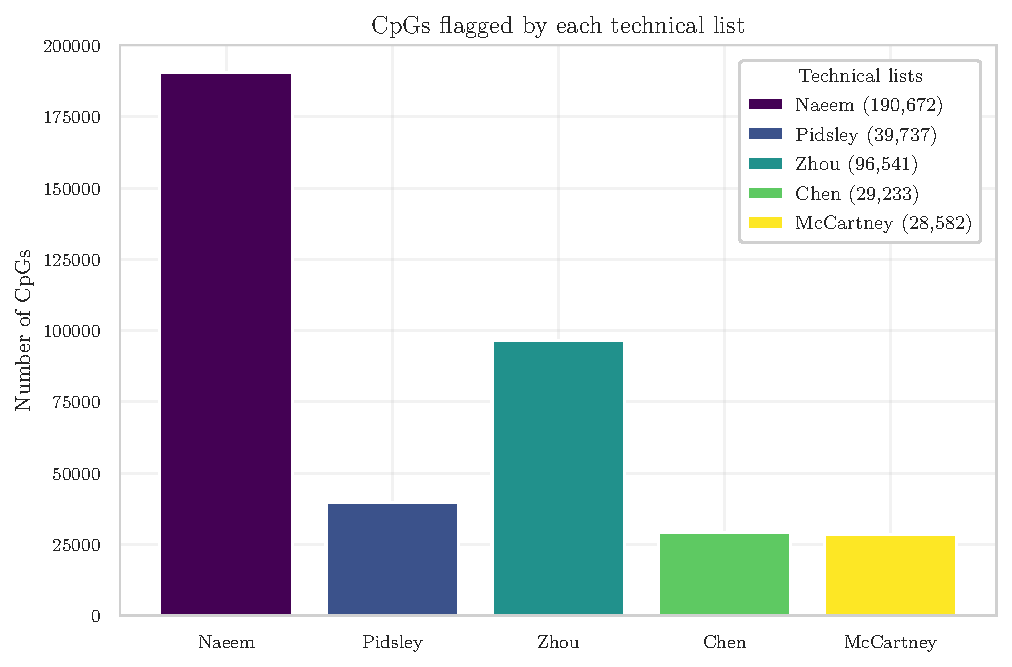
\includegraphics[width=\linewidth]{images/cap4/GSE69914_technical_lists_barplot.pdf}
        \caption{
            CpGs flagged by each technical list. 
        }
        \label{fig:gse69914_tech_barplot}
    \end{subfigure}
    \hfill
    % Panel (b)
    \begin{subfigure}[t]{0.48\linewidth}
        \centering
        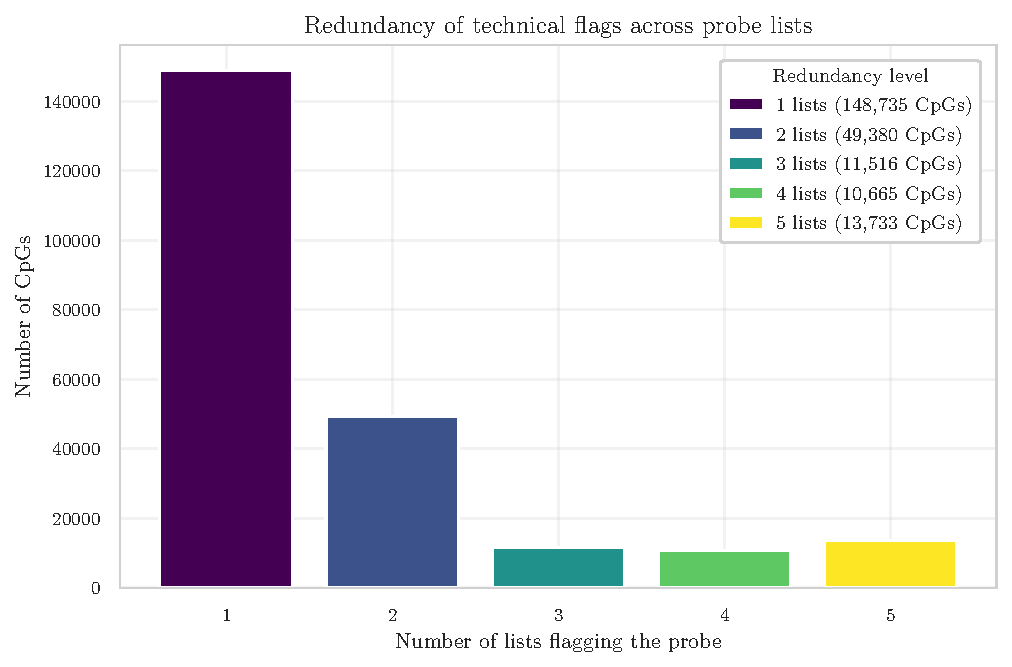
\includegraphics[width=\linewidth]{images/cap4/GSE69914_technical_lists_redundancy_histogram.pdf}
        \caption{Redundancy across filtering lists.}
        \label{fig:gse69914_tech_redundancy}
    \end{subfigure}

    \caption{Technical filtering summary in GSE69914.}
    \label{fig:gse69914_technical_filtering}
\end{figure}

\begin{table}[t]
\centering
\caption{CpG filtering summary for the GSE69914 dataset.}
\label{tab:gse69914_cpg_filtering}
\scriptsize
\begin{tabular}{c c c c c c c c c}
\hline
Initial CpGs &
Naeem &
Pidsley &
Zhou &
Chen &
McCartney &
Non-CpG &
X/Y &
Final CpGs \\
\hline
485{,}512 &
190{,}672 &
39{,}737 &
96{,}541 &
29{,}233 &
28{,}582 &
875 &
7{,}728 &
251{,}483 \\
\hline
\end{tabular}
\end{table}

Intersection with external technical filtering resources resulted in substantial probe removal, as summarised in Table~\ref{tab:gse69914_cpg_filtering}. The largest individual contributions derive from the Naeem and Zhou annotations, while the remaining resources flag smaller but non-negligible subsets. The redundancy structure across lists is shown in Figure~\ref{fig:gse69914_tech_redundancy}.
Because these catalogues target partially distinct classes of technical artefacts—such as cross-reactivity, SNP interference, and repeat-associated probes—limited overlap across lists is expected. Most excluded CpGs are supported by a single resource, with progressively fewer loci flagged by multiple independent annotations. This pattern reflects complementary rather than redundant filtering criteria, while the subset of probes flagged by several lists indicates concordance for loci exhibiting multiple technical vulnerabilities.

Annotation-based validation using the HumanMethylation450 v1.2 manifest~\cite{Illumina450kManifest} further excluded non-CpG probes and loci lacking reliable genomic annotation. Subsequent removal of sex-chromosome probes (X/Y), consistent with established  preprocessing recommendations in mixed-sex cohorts~\cite{maksimovic2012, Wang2022InterpolatedXY}, ensured a strictly autosomal working set.

A detailed per-probe exclusion summary is available in the project repository at  
\href{https://github.com/elisabettaroviera/THESIS/blob/main/05%20-%20CpG%20list/Removed%20CpGs%20per%20Dataset/removed_cpgs_all_filters_summary_gse69914.csv}
{\texttt{removed\_cpgs\_all\_filters\_summary\_gse69914.csv}}.


\paragraph{Statistical Transformation: $\beta$-to-$M$ Values}
\label{par:gse69914_step4}

% ============================================================
% FIGURES: HISTOGRAMS + MEAN–SD FOR BETA AND M
% ============================================================
\begin{figure}[t]
    \centering

    % ---------------- ROW 1: HISTOGRAMS (Beta, Normal & Adjacent) ----------------
    \begin{subfigure}{0.24\textwidth}
        
\includegraphics[width=\textwidth]{images/cap4/GSE69914_hist_normal_beta.pdf}
        \caption{Normal ($\beta$)}
    \end{subfigure}
    \begin{subfigure}{0.24\textwidth}
        
\includegraphics[width=\textwidth]{images/cap4/GSE69914_hist_adjacent_beta.pdf}
        \caption{Adjacent ($\beta$)}
    \end{subfigure}
    \begin{subfigure}{0.24\textwidth}
        
\includegraphics[width=\textwidth]{images/cap4/GSE69914_hist_normal_m.pdf}
        \caption{Normal ($M$)}
    \end{subfigure}
    \begin{subfigure}{0.24\textwidth}
        
\includegraphics[width=\textwidth]{images/cap4/GSE69914_hist_adjacent_m.pdf}
        \caption{Adjacent ($M$)}
    \end{subfigure}

    \vspace{0.8em}

    % ---------------- ROW 2: MEAN–SD RELATIONS ----------------
    \begin{subfigure}{0.24\textwidth}
        
\includegraphics[width=\textwidth]{images/cap4/GSE69914_msd_normal_beta.pdf}
        \caption{Mean–SD Normal ($\beta$)}
    \end{subfigure}
    \begin{subfigure}{0.24\textwidth}
        
\includegraphics[width=\textwidth]{images/cap4/GSE69914_msd_adjacent_beta.pdf}
        \caption{Mean–SD Adjacent ($\beta$)}
    \end{subfigure}
    \begin{subfigure}{0.24\textwidth}
        
\includegraphics[width=\textwidth]{images/cap4/GSE69914_msd_normal_m.pdf}
        \caption{Mean–SD Normal ($M$)}
    \end{subfigure}
    \begin{subfigure}{0.24\textwidth}
        
\includegraphics[width=\textwidth]{images/cap4/GSE69914_msd_adjacent_m.pdf}
        \caption{Mean–SD Adjacent ($M$)}
    \end{subfigure}

    \caption{Distributional comparison of $\beta$ and $M$ in Normal and Adjacent tissues in GSE69914.}
    \label{fig:hist_msd_beta_m}
\end{figure}

Following transformation, the empirical distributions confirm the expected variance-stabilising behaviour of $M$-values (Figure~\ref{fig:hist_msd_beta_m}). In $\beta$-space, both Normal and Adjacent tissues exhibit the characteristic bounded, U-shaped distribution with accumulation near 0 and 1. After logit transformation, the corresponding $M$-value distributions become substantially more symmetric and centered, while preserving the relative structure between tissue groups.
The mean–SD relationships further illustrate the scale effect. In $\beta$-space, variance is strongly mean-dependent and inflates near intermediate methylation levels, producing a pronounced curvature in the mean–SD plots. In contrast, $M$-values display markedly flatter dispersion profiles across the full range, indicating substantial reduction of heteroscedasticity. 

This behaviour is fully consistent with the theoretical and empirical findings of Du et al.~\cite{Du2010}, which motivate the use of $M$-values for inferential modelling.


% ============================================================

\subsection{Dataset GSE225845}
\label{subsec:gse225845_preproc}
% ============================================================

\paragraph{Structural Integrity and Cohort Harmonization}
\label{par:gse225845_step0}

The dataset comprised 477 samples and 750{,}426 CpGs at load time, consistent with the dimensionality of the Illumina EPIC platform.  
The phenotype table contained 477 entries, and alignment between phenotype annotation and the $\beta$-value matrix was exact. No duplicated entries were detected, and all required metadata fields were present.

Probe-level and sample-level missingness assessment confirmed that the methylation matrix was fully observed.  
No missing CpG values and no incomplete samples were detected. Consequently, no imputation or early NaN filtering was required prior to probe-type bias diagnostics and technical filtering.


\paragraph{Probe-Type Bias Diagnostics and Correction}
\label{par:gse225845_step1}
\begin{figure}[t]
    \centering
    \begin{subfigure}[t]{0.48\linewidth}
        \centering
        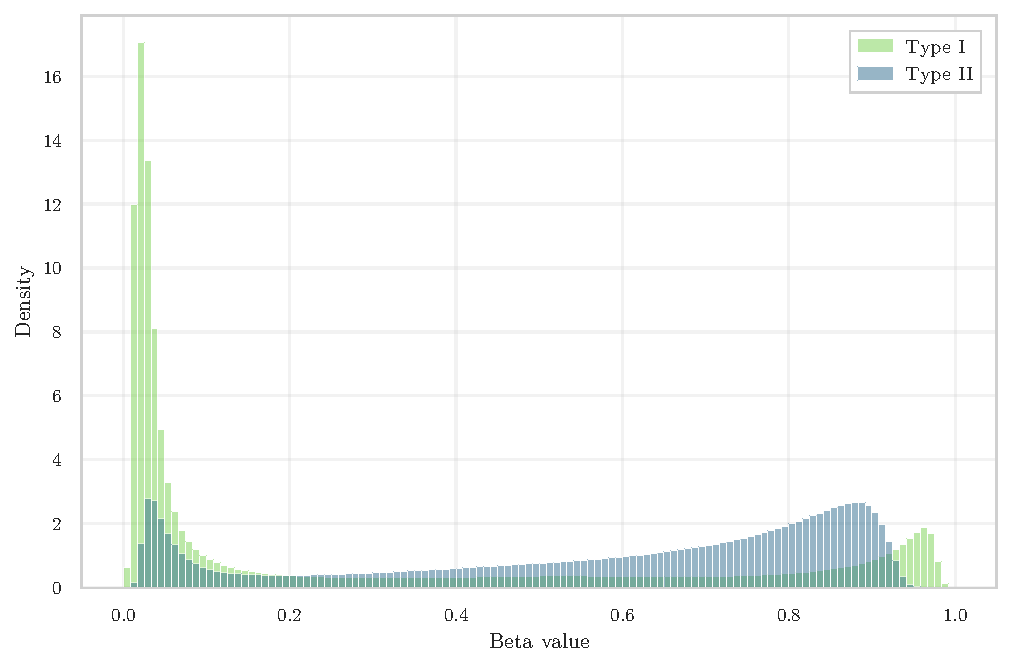
\includegraphics[height=4.5cm,keepaspectratio]{images/cap4/GSE225845_type_bias_density.pdf}
        \caption{$\beta$-value density by probe type.}
        \label{fig:GSE225845_type_bias_density}
    \end{subfigure}
    \hfill
    \begin{subfigure}[t]{0.48\linewidth}
        \centering
        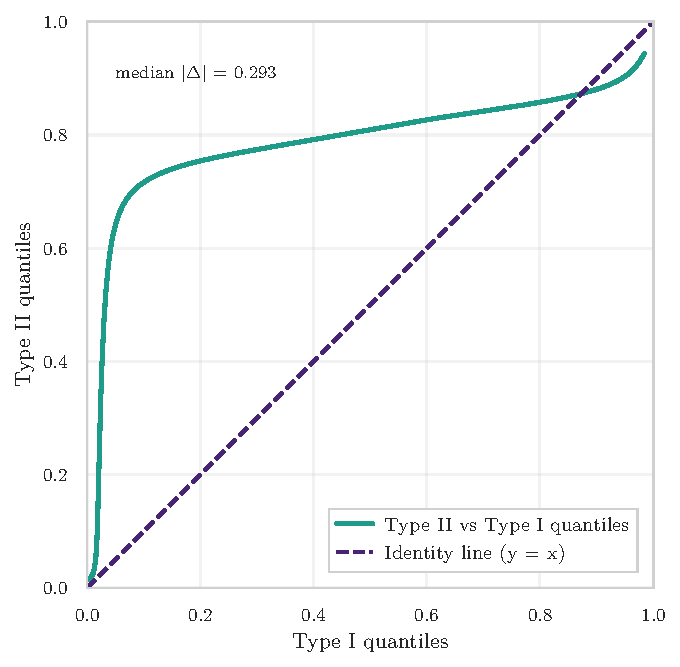
\includegraphics[height=4.5cm,keepaspectratio]{images/cap4/GSE225845_type_bias_qqplot.pdf}
        \caption{Q--Q plot (Type~II vs.~Type~I).}
        \label{fig:GSE225845_type_bias_qq}
    \end{subfigure}
    \caption{Infinium Type~I/II bias diagnostics in GSE225845.}
    \label{fig:type_bias_combined}
\end{figure}

Stratification by probe design yielded 119{,}760 Type~I and 627{,}842 Type~II probes.  
Raw intensity data were reported by the original authors to have been processed using the \texttt{minfi} pipeline with BMIQ normalization (v1.4)~\cite{GSE225845}.
The $\beta$-value density distributions (Figure~\ref{fig:GSE225845_type_bias_density}) show substantial overlap between probe families. Type~I probes retain the characteristic concentration near the unmethylated and fully methylated boundaries, while Type~II probes display a broader distribution; however, no pronounced multimodal distortion or systematic separation is observed.
Quantile--quantile analysis (Figure~\ref{fig:GSE225845_type_bias_qq}) further supports this interpretation. Although minor deviations from the identity line ($y = x$) are visible, the overall alignment indicates largely balanced probe-type scaling. The median absolute deviation $\mathrm{median}|\Delta| = 0.293$ suggests that probe-type differences are attenuated but not entirely eliminated, consistent with residual variation commonly observed after BMIQ normalization~\cite{Teschendorff2013BMIQ, maksimovic2012, Wang2015Normalization450K}.

Overall, the diagnostic patterns are compatible with prior application of probe-type bias correction.

\paragraph{Technical Probe Filtering}
\label{par:gse225845_step2}

\begin{figure}[t]
    \centering

    % Panel (a)
    \begin{subfigure}[t]{0.48\linewidth}
        \centering
        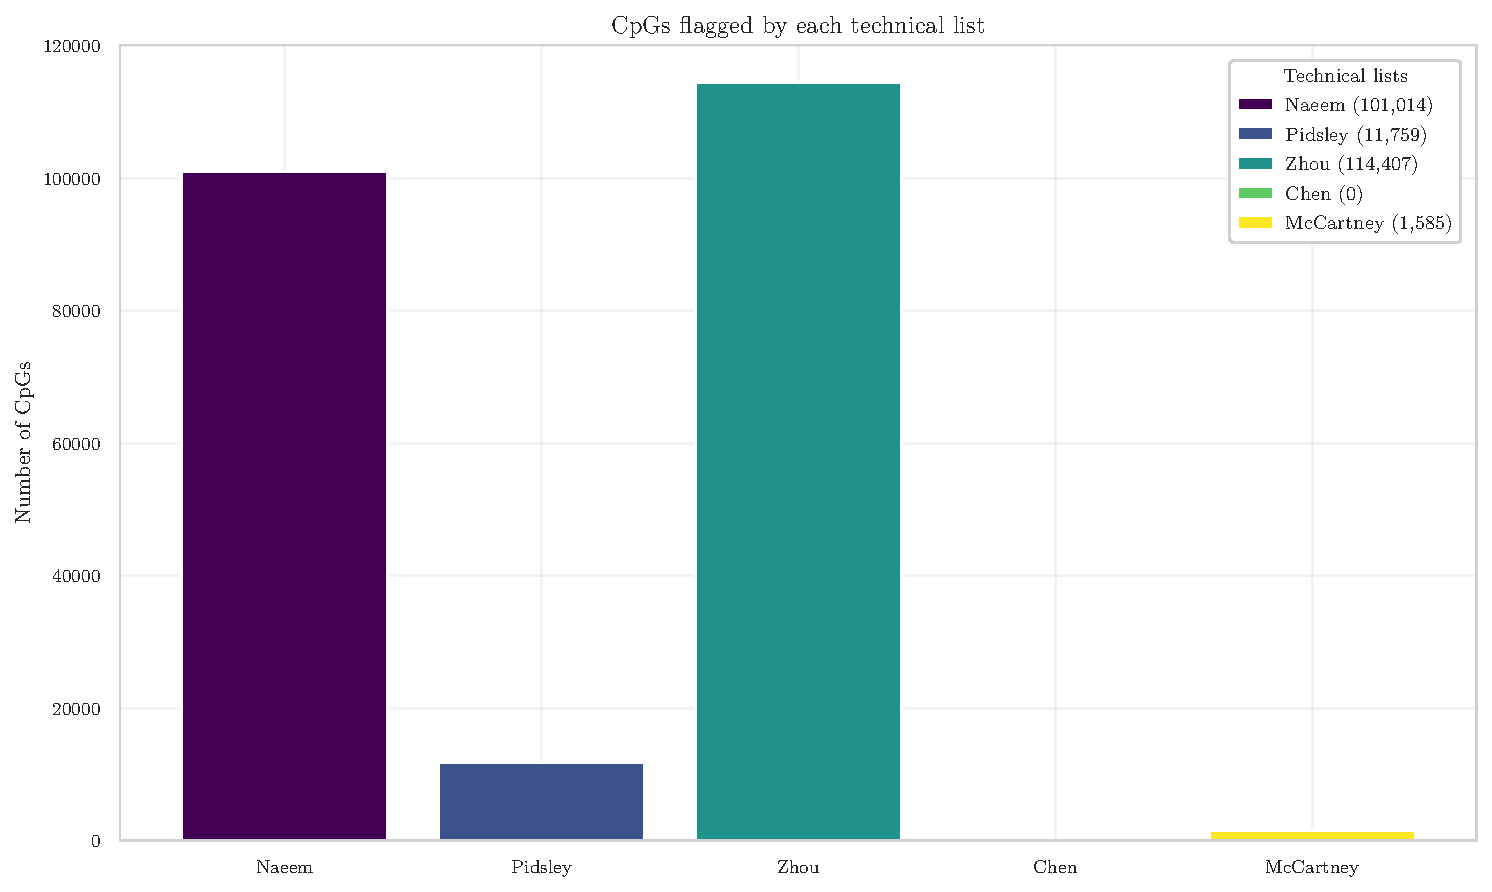
\includegraphics[width=\linewidth]{images/cap4/GSE225845_technical_lists_histogram.pdf}
        \caption{
            CpGs flagged by each technical list. 
        }
        \label{fig:gse225845_tech_barplot}
    \end{subfigure}
    \hfill
    % Panel (b)
    \begin{subfigure}[t]{0.48\linewidth}
        \centering
        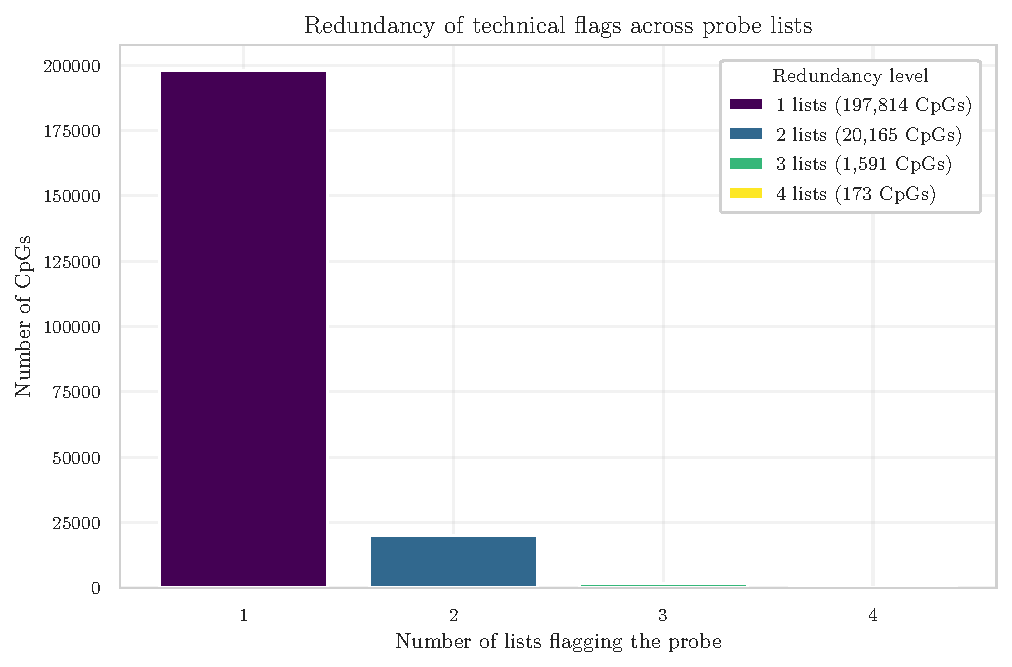
\includegraphics[width=\linewidth]{images/cap4/GSE225845_technical_lists_redundancy_histogram.pdf}
        \caption{Redundancy across filtering lists.}
        \label{fig:gse225845_tech_redundancy}
    \end{subfigure}

    \caption{Technical filtering summary in GSE225845.}
    \label{fig:gse225845_technical_filtering}
\end{figure}

Intersection with external technical filtering resources resulted in substantial probe removal, as summarised in Table~\ref{tab:gse225845_cpg_filtering}. The largest individual contributions derive from the Zhou and Naeem annotations, while the remaining resources flag smaller subsets. The redundancy structure across lists is shown in Figure~\ref{fig:gse225845_tech_redundancy}.
A detailed per-probe exclusion summary is available in the project repository at  
\href{https://github.com/elisabettaroviera/THESIS/blob/main/05%20-%20CpG%20list/Removed%20CpGs%20per%20Dataset/removed_cpgs_all_filters_summary_gse225845.csv}
{\texttt{removed\_cpgs\_all\_filters\_summary\_gse225845.csv}}.
\begin{table}[t]
\centering
\caption{CpG filtering summary for the GSE225845 dataset.}
\label{tab:gse225845_cpg_filtering}
\scriptsize
\begin{tabular}{c c c c c c c c c}
\hline
Initial CpGs &
Naeem &
Pidsley &
Zhou &
Chen &
McCartney &
Non-CpG &
X/Y &
Final CpGs \\
\hline
750{,}426 &
101{,}014 &
11{,}759 &
114{,}407 &
0 &
1{,}585 &
773 &
14{,}071 &
530{,}683 \\
\hline
\end{tabular}
\end{table}

\paragraph{Statistical Transformation: $\beta$-to-$M$ Values}
\label{par:gse225845_step3}

\begin{figure}[t]
    \centering

    % ---------------- ROW 1: HISTOGRAMS ----------------
    \begin{subfigure}{0.24\textwidth}
        
\includegraphics[width=\textwidth]{images/cap4/GSE225845_hist_normal_beta.pdf}
        \caption{Normal ($\beta$)}
    \end{subfigure}
    \begin{subfigure}{0.24\textwidth}
        
\includegraphics[width=\textwidth]{images/cap4/GSE225845_hist_adjacent_beta.pdf}
        \caption{Adjacent ($\beta$)}
    \end{subfigure}
    \begin{subfigure}{0.24\textwidth}
        
\includegraphics[width=\textwidth]{images/cap4/GSE225845_hist_normal_m.pdf}
        \caption{Normal ($M$)}
    \end{subfigure}
    \begin{subfigure}{0.24\textwidth}
        
\includegraphics[width=\textwidth]{images/cap4/GSE225845_hist_adjacent_m.pdf}
        \caption{Adjacent ($M$)}
    \end{subfigure}

    \vspace{0.3cm}

    % ---------------- ROW 2: MEAN–SD RELATIONS ----------------
    \begin{subfigure}{0.24\textwidth}
        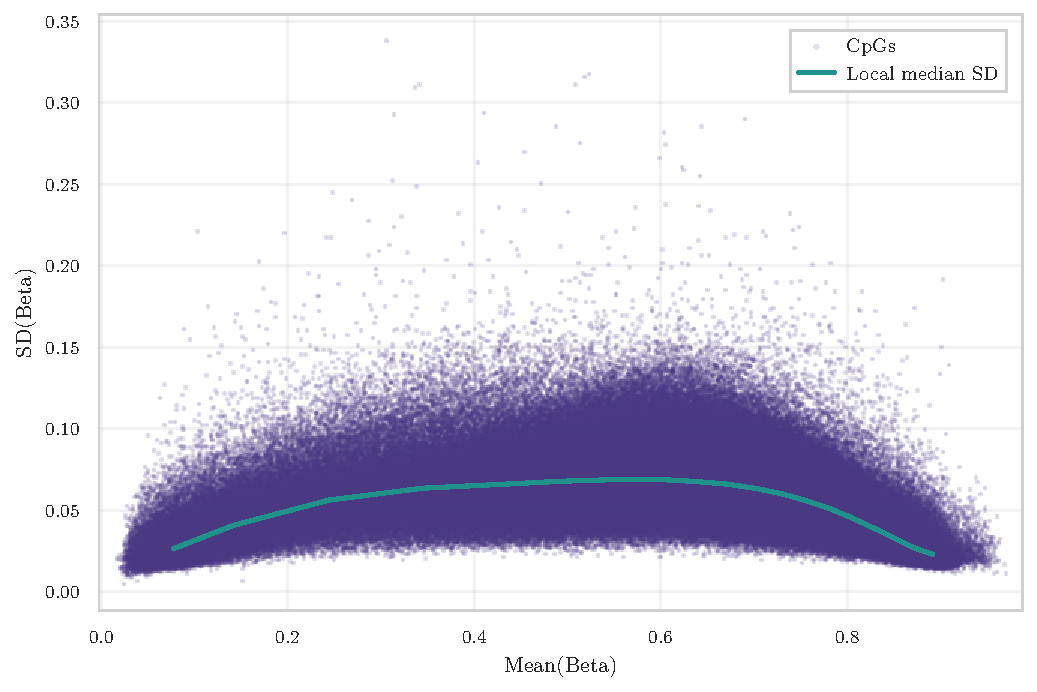
\includegraphics[width=\textwidth]{images/cap4/GSE225845_msd_normal_beta.pdf}
        \caption{Mean–SD Normal ($\beta$)}
    \end{subfigure}
    \begin{subfigure}{0.24\textwidth}
        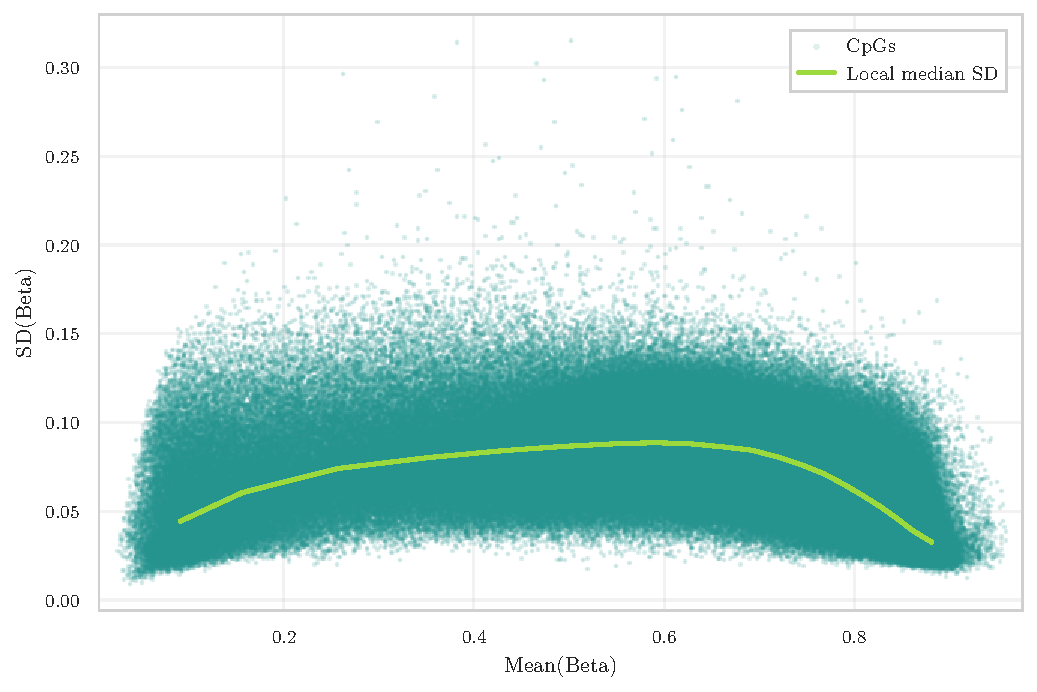
\includegraphics[width=\textwidth]{images/cap4/GSE225845_msd_adjacent_beta.pdf}
        \caption{Mean–SD Adjacent ($\beta$)}
    \end{subfigure}
    \begin{subfigure}{0.24\textwidth}
        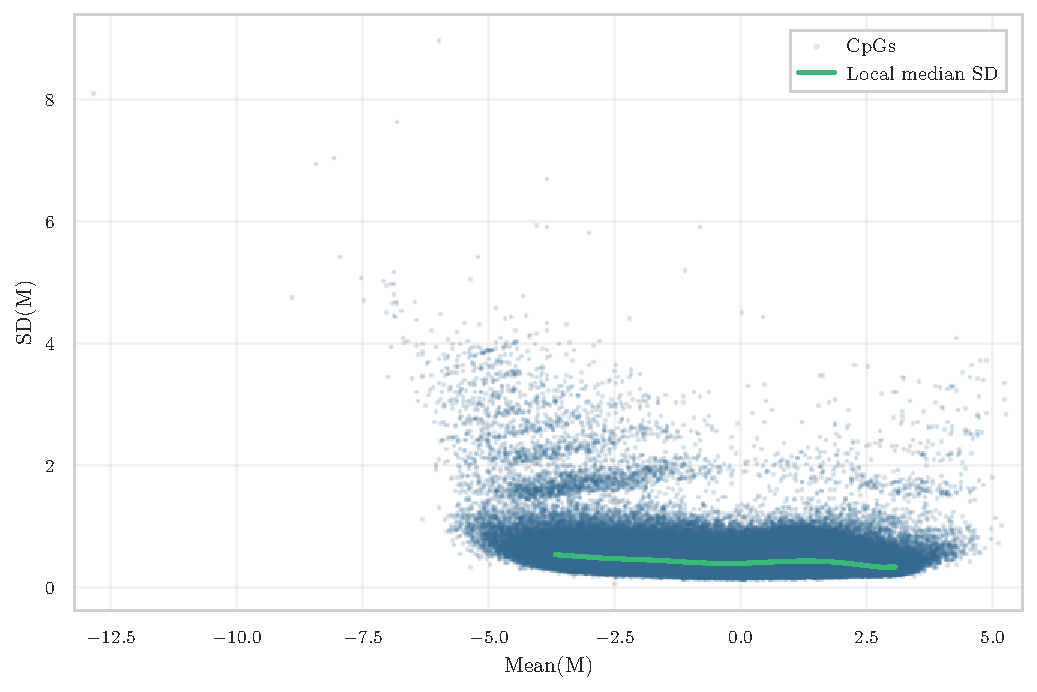
\includegraphics[width=\textwidth]{images/cap4/GSE225845_msd_normal_m.pdf}
        \caption{Mean–SD Normal ($M$)}
    \end{subfigure}
    \begin{subfigure}{0.24\textwidth}
        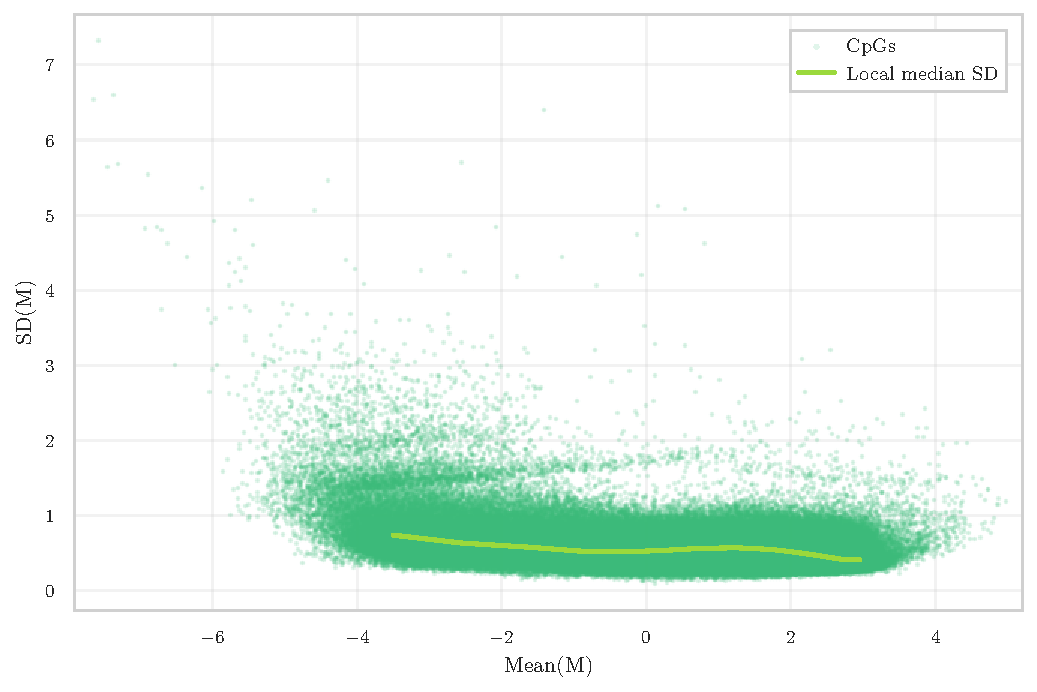
\includegraphics[width=\textwidth]{images/cap4/GSE225845_msd_adjacent_m.pdf}
        \caption{Mean–SD Adjacent ($M$)}
    \end{subfigure}

    \caption{Distributional comparison of $\beta$ and $M$ in Normal and Adjacent
tissues in GSE225845.}
    \label{fig:gse225845_beta_m_combined}
\end{figure}

All filtered $\beta$-values were transformed to $M$-values using the logit relation defined in Equation~\eqref{eq:mvalue}. 
The empirical distributions (Figure~\ref{fig:gse225845_beta_m_combined}) show the characteristic bounded, U-shaped profile in $\beta$-space for both Normal and Adjacent tissues. After transformation, the corresponding $M$-value distributions become substantially more symmetric and centered, while maintaining the relative structure between tissue classes.

The mean--SD relationships further illustrate the scale effect. In $\beta$-space, variance exhibits pronounced mean dependence, with inflation at intermediate methylation levels and compression near the boundaries. In contrast, $M$-values display markedly flatter dispersion profiles across the full range, indicating substantial reduction of heteroscedasticity. 


% ============================================================
\subsection{Dataset GSE287331}
\label{subsec:gse287331_data_prep}
% ============================================================

DESCRIZIONE BMIQ IMPLEMENTATION
For GSE287331, BMIQ correction is implemented strictly on a per-sample basis. 
The Infinium probe-type annotation is derived from the official EPIC manifest, 
and the design vector is aligned to the CpG ordering of the $\beta$-matrix 
prior to correction. Within each sample, Type~I probes define the reference 
mixture distribution, and Type~II probes are rescaled accordingly; no 
cross-sample or cross-group information is introduced at any stage. 
Samples with insufficient numbers of probes per design type are left 
uncorrected to avoid unstable mixture estimation. This implementation 
ensures that probe-type bias is addressed without altering between-sample 
structure or introducing artificial harmonisation across tissue classes.

% ============================================
% Missingness
% ============================================
\paragraph{Missingness filtering and imputation}
\label{par:gse287331_missingness}
I quantified the amount and structure of
missing values in the $\beta$-matrix. Probe-wise missingness is a well-known
source of unreliability in Illumina methylation arrays, and several studies recommend
removing CpGs that exhibit low measurement quality or an excessive proportion of missing
values. For example, Islam \textit{et al.}~\cite{islam2019_pediatric_dnamm} excluded probes
with missing $\beta$-values in more than $2\%$ of samples in their pediatric tissue
methylation analysis, while Mansell \textit{et al.}~\cite{mansell2019guidance} applied a
similar $1\%$ threshold for detection failure in their EPIC-array quality control
pipeline. 

Guided by this evidence and the large number of CpG sites available,
I adopted a stringent probe-wise filtering criterion and removed all
CpGs missing in more than $1\%$ of samples. This choice prioritises high-confidence
measurements while minimising reliance on imputed values.

After filtering, only a negligible fraction of values remained missing in the working
matrix (58\,561 NaN, corresponding to $0.0187\%$ of all entries). Given this extremely low
level of sparsity, median-based imputation is both statistically robust and
distribution-preserving. Following current recommendations, where missing methylation values
are replaced by probe-wise medians to avoid introducing group-specific bias, all residual
NaN were imputed using the median $\beta$-value of each CpG across samples. This approach is consistent with recent harmonization methods such as mLiftOver, 
where missing methylation values are explicitly replaced using probe-wise median 
substitution to preserve biologically plausible levels \cite{chen2024_mliftover}.


% Giustificazione evidence che non e' stato fatto BMIQ
\paragraph{Evidence of Missing Infinium Type~I/II Probe Bias Correction}

During the exploratory analysis performed uniformly across all three datasets, the per-sample
mean $\beta$-value distributions (Fig.~\ref{fig:gse287331_mean_beta_1}, 
Fig.~\ref{fig:gse287331_mean_beta_2}, 
Fig.~\ref{fig:gse287331_mean_beta_3_pre})
revealed a marked inconsistency.  
Whereas \texttt{GSE69914} and \texttt{GSE225845} displayed a single broad peak of global
methylation levels, \texttt{GSE287331} showed a much narrower distribution, shifted towards
higher $\beta$-values and characterized by two distinct modes in the high-$\beta$ range.

This unusual right-shifted bimodality---largely absent in the other datasets---strongly indicated 
that a key preprocessing step, namely Infinium Type~I/II probe-design bias correction, had not 
been applied in the processed data released by the authors.

\begin{figure}[t]
    \centering
    \begin{subfigure}{0.24\textwidth}
        \centering
        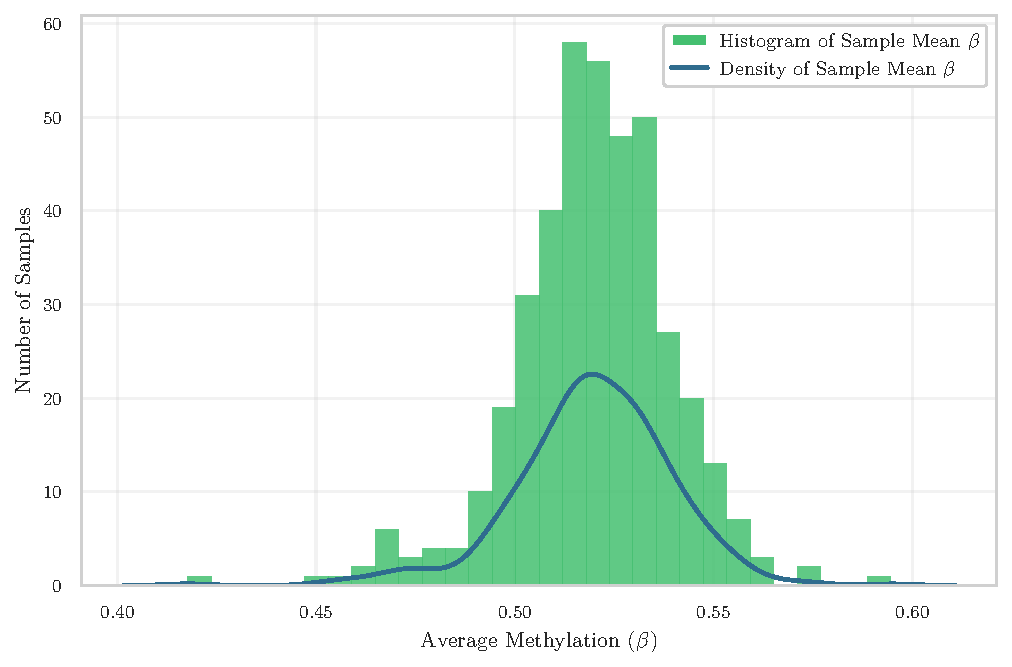
\includegraphics[width=\textwidth]{images/cap3/GSE69914_08_mean_beta_per_sample.pdf}
        \caption{GSE69914}
        \label{fig:gse287331_mean_beta_1}
    \end{subfigure}
    \hfill
    \begin{subfigure}{0.24\textwidth}
        \centering
        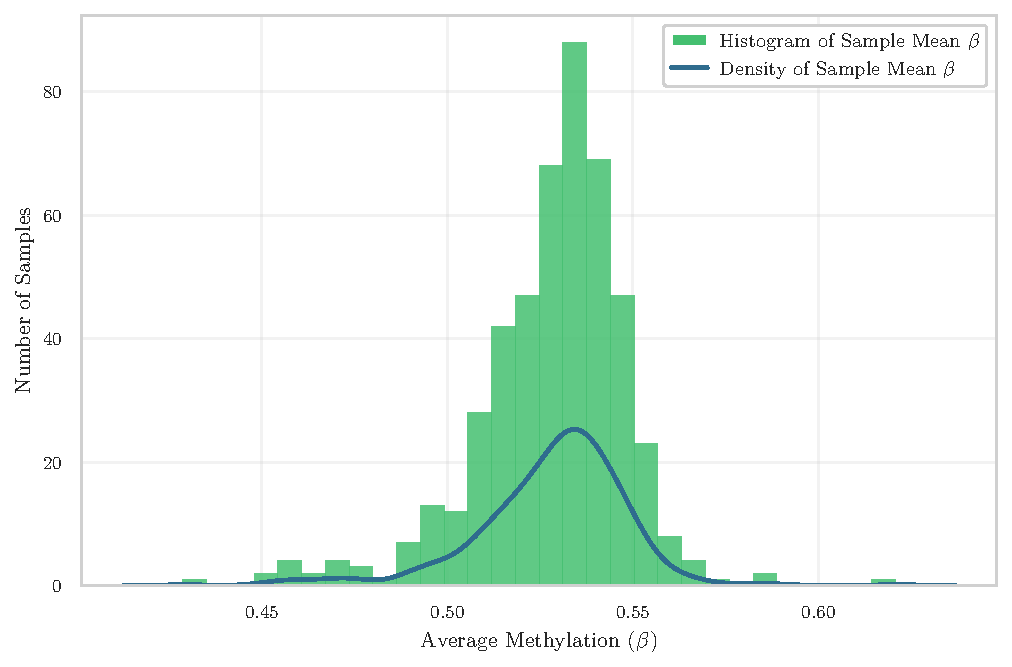
\includegraphics[width=\textwidth]{images/cap3/GSE225845_08_mean_beta_per_sample.pdf}
        \caption{GSE225845}
        \label{fig:gse287331_mean_beta_2}
    \end{subfigure}
    \hfill
    \begin{subfigure}{0.24\textwidth}
        \centering
        
\includegraphics[width=\textwidth]{images/cap3/GSE287331_08_mean_beta_per_sample.pdf}
        \caption{GSE287331 pre BMIQ}
        \label{fig:gse287331_mean_beta_3_pre}
    \end{subfigure}
    \hfill
    \begin{subfigure}{0.24\textwidth}
        \centering
        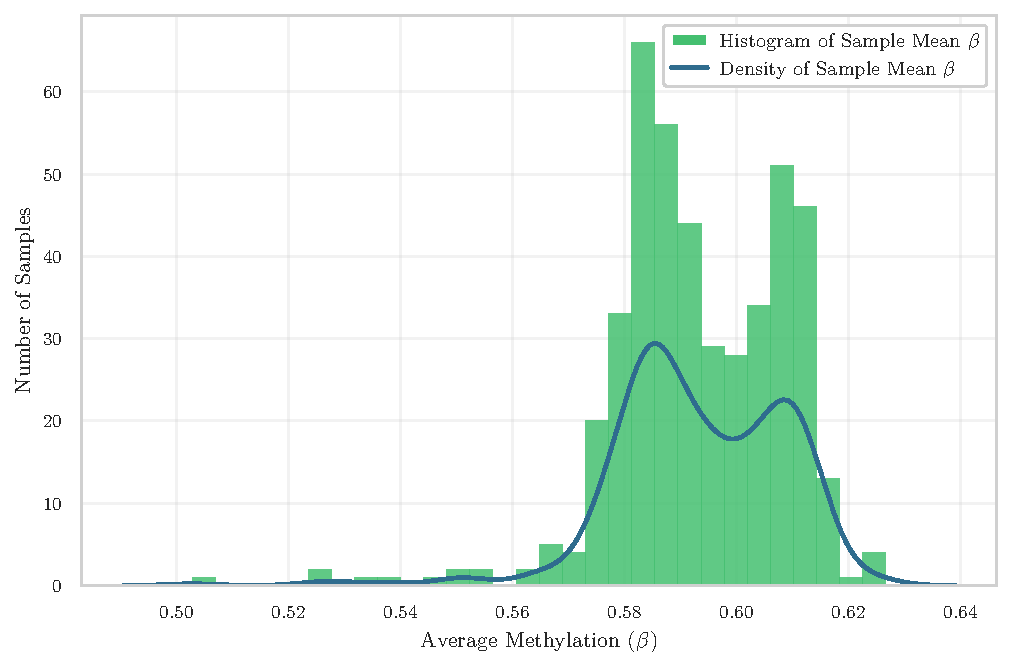
\includegraphics[width=\textwidth]{images/cap3/GSE287331_03_mean_beta_per_sample.pdf}
        \caption{GSE287331 post BMIQ}
        \label{fig:gse287331_mean_beta_3_post}
    \end{subfigure}
    \caption{Per-sample mean $\beta$ distributions for the three datasets. 
    \texttt{GSE69914} and \texttt{GSE225845} show a single broad peak, whereas 
    \texttt{GSE287331} displays a right-shifted bimodal pattern. After BMIQ, the two peaks 
    become slightly closer and more similar in height, but the bimodality persists.}
    \label{fig:mean_beta_comparison_three}
\end{figure}

To confirm this hypothesis, I stratified all probes by Infinium design type (Type~I vs.~Type~II) 
using the official Illumina EPIC v1.0 manifest, obtained from the corresponding Bioconductor 
annotation package \cite{Illumina450kAnno}. Using this manifest, the $\beta$-value distributions 
were separated by probe design and inspected through a dedicated diagnostic plot 
(Fig.~\ref{fig:gse287331_type_bias_check}). According to the expected behaviour described by 
Teschendorff et~al.~\cite{Teschendorff2013BMIQ}, datasets that have undergone BMIQ
normalization should display nearly overlapping $\beta$-value distributions for the two probe types.

In contrast, the Q--Q plot comparing Type~I and Type~II probes revealed a markedly elevated 
median absolute deviation (median $|\Delta| = 0.380$), indicating a strong and systematic 
quantile-wise shift between the two designs. Such a deviation is fully incompatible with 
BMIQ-corrected data, which should instead exhibit deviations close to zero across all quantiles.  
After applying BMIQ, this deviation decreases only marginally ($|\Delta| : 0.380 \rightarrow 0.370$), 
confirming that the correction improves probe-type alignment but only to a limited extent.

This modest improvement is also clearly visible in the diagnostic density plots 
(Fig.~\ref{fig:gse287331_typeI_II_post}). After BMIQ, the rightmost portion of the distribution 
(near $\beta \approx 1$) shows Type~II probes becoming visibly more similar to Type~I, and the 
strong asymmetry between the two curves is partially reduced. Nevertheless, the overall shapes 
of the two probe distributions remain distinct, and the characteristic ``double-tail’’ pattern 
of the uncorrected dataset is still present after normalization. BMIQ therefore warps the 
distribution in the expected direction, but the magnitude of the adjustment is small and 
insufficient to reconcile the two probe types to the degree observed in datasets processed with 
a full bias-correction pipeline.

A similar behaviour can be observed in the per-sample mean $\beta$ distributions: after BMIQ, the 
two peaks become slightly higher and closer to one another 
(Fig.~\ref{fig:gse287331_mean_beta_3_post}), indicating that the algorithm partially reduces the 
gap between the two dominant modes. However, even after correction, the distribution remains 
visibly and consistently \emph{bimodal}, suggesting that BMIQ mitigates only weakly the underlying 
discrepancy and that sample-level heterogeneity continues to dominate the global methylation 
structure.

Taken together, these observations provide clear visual evidence that no probe-design bias 
correction was applied in the original processing. To further support this conclusion, 
I examined the official publication~\cite{Lord2024GSE287331}. The paper carefully describes the acquisition, 
processing, and analytical use of Illumina EPIC $\beta$-values, but it does \emph{not} mention 
BMIQ, SWAN, noob, or any other method aimed at correcting Infinium probe-type bias.  
The absence of such a statement---combined with the strong visual mismatch between Type~I and 
Type~II probe distributions---confirms that no probe-design bias correction was applied before the 
release of the dataset.

For these reasons, applying a dedicated Infinium Type~I/II bias correction step is necessary 
before performing any comparative analysis.

\begin{figure}[t]
    \centering
    \begin{subfigure}{0.49\textwidth}
        \centering
        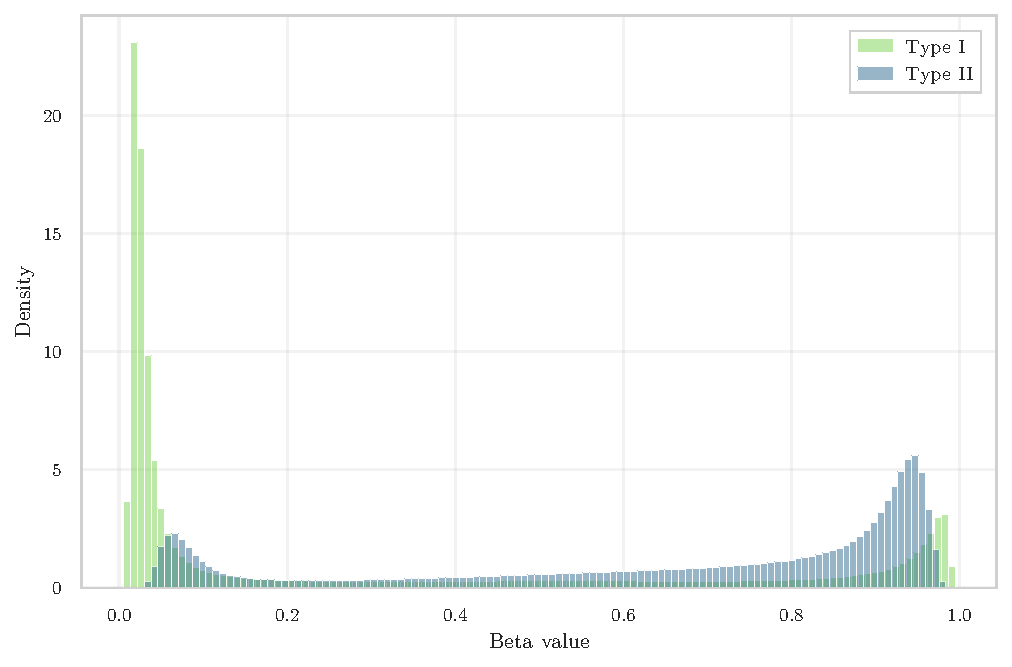
\includegraphics[width=\textwidth]{images/cap3/GSE287331_23_type_bias_density_pre.pdf}
        \caption{GSE287331 pre BMIQ}
        \label{fig:gse287331_typeI_II_pre}
    \end{subfigure}
    \hfill
    \begin{subfigure}{0.49\textwidth}
        \centering
        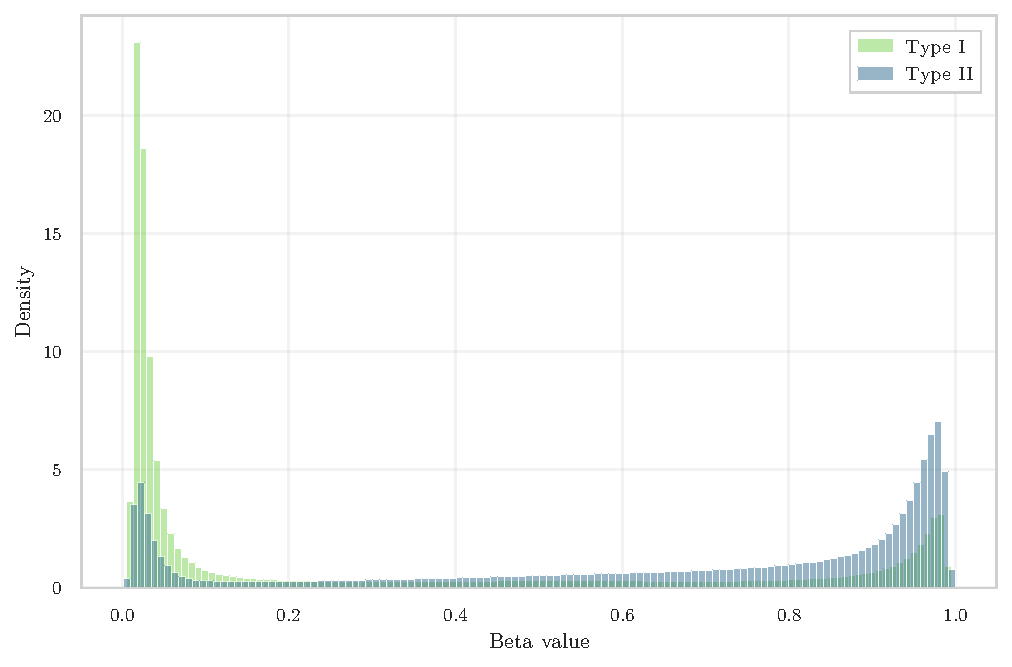
\includegraphics[width=\textwidth]{images/cap3/GSE287331_23_type_bias_density_post.pdf}
        \caption{GSE287331 post BMIQ}
        \label{fig:gse287331_typeI_II_post}
    \end{subfigure}
    \caption{Type~I vs.~Type~II probe design comparison before and after BMIQ.  
    After correction, Type~II probes become more similar to Type~I in the high-$\beta$ region
    (especially near $\beta \approx 1$), and the overall discrepancy is reduced 
    ($|\Delta| : 0.380 \rightarrow 0.370$), though probe types remain clearly distinct.}
    \label{fig:gse287331_type_bias_check}
\end{figure}

\paragraph{BMIQ correction: implementation and methodological considerations}
\label{par:gse287331_bmiq}

Given the clear evidence of missing Infinium Type~I/II probe-bias correction, 
I applied the canonical BMIQ algorithm
\cite{Teschendorff2013BMIQ}, using the implementation provided by the 
\texttt{wateRmelon} package \cite{Pidsley2013wateRmelon}, to harmonize the 
distributions of Type~I and Type~II probes for each sample. To ensure full 
reproducibility and strict memory control on the extremely wide EPIC matrix, I implemented a \emph{sequential, sample-wise BMIQ correction}, 
avoiding any between-sample pooling or multi-core parallelization. Each sample’s 
$\beta$ vector was processed independently using a safe wrapper around 
\texttt{wateRmelon::BMIQ}, which first verified the availability of a sufficient 
number of non-missing Type~I and Type~II probes and then returned the corrected 
$\beta$-values. The corrected matrix was updated in place, preserving the schema 
\texttt{id\_tissue | CpGs... | label} and subsequently written to a single Parquet file. 
This design guarantees that no cross-sample information influenced the correction and 
that the warping applied by BMIQ reflects exclusively the distributional 
characteristics of each individual sample.

While BMIQ is widely used to mitigate probe-design bias, multiple studies have raised
important methodological caveats regarding normalization procedures that operate on
the full distribution of methylation values. Yousefi \textit{et al.}~\cite{Yousefi2013Normalization}
highlighted that quantile-based adjustments and related normalization strategies
may ``come at the cost of \emph{artificially reduced biological variability},'' 
a phenomenon that is particularly undesirable when studying biological groups expected 
to differ globally in their methylation profiles. Similarly, Liu \textit{et al.}
\cite{Liu2016Processing} reported that, when methylation alterations are extensive in size
and number, certain normalization methods can ``\emph{remove biological signal},'' 
effectively shrinking meaningful differences between groups. 

More recently, Welsh \textit{et al.}~\cite{Welsh2023EPICnorm} performed a systematic
evaluation of normalization methods for EPIC arrays and showed that approaches enforcing
strong distributional alignment may distort real biological structure. In particular,
the authors observed that quantile-based normalization ``\emph{forces the empirical 
marginal distributions of the samples to be the same, removing all variation in this
statistic},'' and reported that BMIQ, in some settings, yielded ``\emph{distorted and 
discontinuous}'' distributions. Such findings provide a conceptual explanation for the 
behaviour observed: although BMIQ was applied strictly 
per-sample, its within-array warping can attenuate global differences between 
Normal, Adjacent, and Tumor samples when these differences are manifested as broad 
shifts in the underlying $\beta$-value distribution.

Together, these considerations emphasise both the necessity and the limitations of
probe-design bias correction. Applying BMIQ was essential to remove the technical 
Type~I/II bias absent in the original processing, yet its known 
tendency to reduce distributional heterogeneity across groups must be carefully taken 
into account when interpreting group-level contrasts in downstream analyses.

Importantly, the modest degree of probe-type harmonization is accompanied by a noticeable 
flattening of biological structure: as will be shown in the low-dimensional embedding analysis 
(Section~\ref{par:gse287331_embeddings}), PCA, UMAP, and t-SNE projections reveal that the 
Normal, Adjacent, and Tumor groups become \emph{less clearly separable} after BMIQ.  
For this reason, all downstream analyses are carried out on the \textbf{non-BMIQ version} of the 
dataset, which preserves sharper cluster boundaries and better reflects the underlying biological 
signal.

This strong separation is also quantitatively confirmed by silhouette analysis:  
the average silhouette coefficient \emph{before} BMIQ was 
$\mathrm{sil}_{\text{pre}} = 0.2876$,  
but \emph{after} BMIQ correction it declined to 
$\mathrm{sil}_{\text{post}} = 0.2537$.  
Thus, BMIQ \emph{reduced}--even if not significantly--the natural clusterability of the data, collapsing genuine 
biological differences—particularly the clear separation between Normal and Adjacent 
samples.

For this reason, and in accordance with the principle of preserving authentic biological 
signal, the BMIQ-normalised version was not adopted.  


\paragraph{Step~0 -- Initial Pre-processing}
\label{par:gse287331_step0}

The dataset was imported from its Parquet representation, yielding an initial
$\beta$-value matrix of 446 samples and 866{,}552 CpGs.
The accompanying phenotype table reported the same number of entries and contained
all required metadata fields.  
Before continuing with probe-level preprocessing, the dataset underwent a dedicated
missingness-cleaning stage to ensure high-quality input for downstream analysis.
After harmonising phenotype labels and applying dataset-specific selection rules, only samples belonging to the three core tissue states of interest—Normal, Adjacent, and Tumour—were kept.
This resulted in a final working cohort of 311 samples, used for all downstream preprocessing and analysis.

\textbf{Missingness filtering and imputation.}
Probe-wise missingness was quantified across the $\beta$-matrix.  
Consistent with recommendations from Islam \textit{et al.}~\cite{islam2019_pediatric_dnamm}
and Mansell \textit{et al.}~\cite{mansell2019guidance}, a stringent threshold was applied:
all CpG sites missing in more than 1\% of samples were removed.
This filter ensures high-confidence measurements while leveraging the
large dimensionality of the EPIC platform.

After applying this criterion, the remaining level of sparsity was extremely low,
with only 58{,}561 NaN values (0.0187\% of all entries).  
These residual missing values were imputed using probe-wise median substitution,
a strategy that avoids introducing group-specific bias and is also adopted in
recent harmonisation workflows such as mLiftOver~\cite{chen2024_mliftover}.

The resulting $\beta$-matrix contained no missing values.

\textbf{Data integrity verification.}
After missingness filtering and imputation, the final working matrix consisted of  
311 samples and 702{,}916 CpGs.  
All entries were fully observed (0 residual NaN).

\paragraph{Step~1 -- Infinium Type I/II Bias Diagnostics}
\label{subpar:gse287331_typebias}

\begin{figure}[t]
    \centering
    \begin{subfigure}[t]{0.49\textwidth}
        \centering
        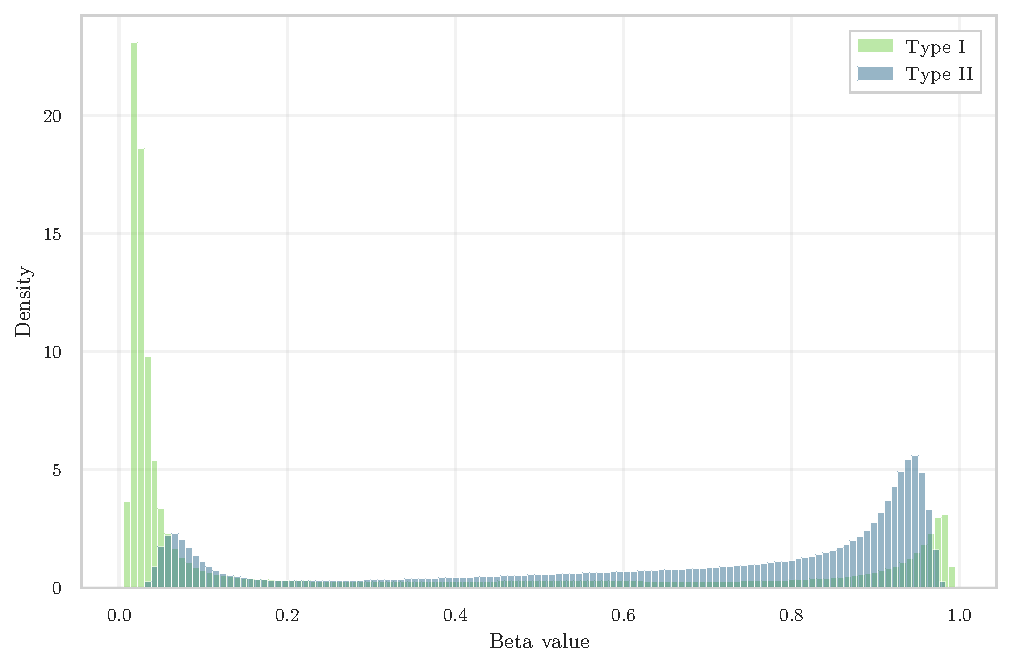
\includegraphics[width=\textwidth]{images/cap4/GSE287331_type_bias_density.pdf}
        \caption{Type~I vs.\ Type~II density (pre BMIQ).}
        \label{fig:gse287331_type_bias_density}
    \end{subfigure}
    \hfill
    \begin{subfigure}[t]{0.49\textwidth}
        \centering
        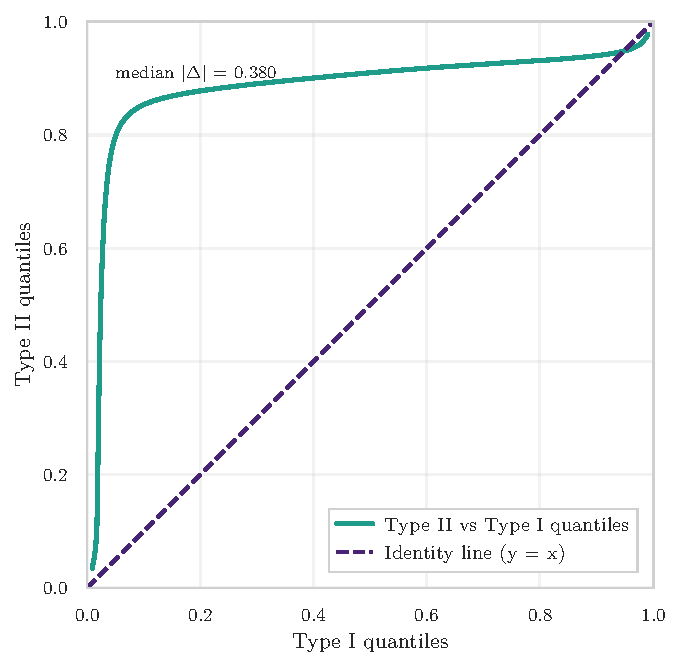
\includegraphics[width=0.68\textwidth]{images/cap4/GSE287331_type_bias_qqplot.pdf}
    \caption{
        Q--Q comparison of Type~II vs.\ Type~I probes (pre BMIQ).  
        The median absolute deviation of 0.380 indicates a strong quantile-wise shift,
        confirming the absence of probe-type normalization in the original dataset.
    }
    \label{fig:gse287331_type_bias_qq}
    \end{subfigure}
    \caption{
        Diagnostic evaluation of Infinium probe–design bias before and after BMIQ.  
        The correction reduces the discrepancy only marginally, and substantial
        distributional differences remain between probe types.
    }
    \label{fig:gse287331_type_bias_combined}
\end{figure}

 Using the official EPIC v1.0 manifest,  
115{,}705 Type~I and 585{,}514 Type~II probes were identified. The $\beta$-value distributions of the two chemistries showed a marked mismatch
(Figure~\ref{fig:gse287331_type_bias_density}), with Type~II probes displaying a strong
right-shifted profile. The quantile--quantile comparison confirmed a substantial systematic
offset, with a median absolute deviation of 0.380
(Figure~\ref{fig:gse287331_type_bias_qq}), indicating the absence of any Infinium
probe-design bias correction in the originally released data.

Given this discrepancy, a per-sample BMIQ normalization step was applied using the
\texttt{wateRmelon} implementation, operating strictly on individual samples to minimise
cross-sample distortion. Post-correction diagnostics showed a modest reduction in
probe-type mismatch ($|\Delta| : 0.380 \rightarrow 0.370$) and a slight improvement in the
alignment of high-$\beta$ regions, but the overall distributional discrepancy remained
substantial. 
Due to this limited harmonization and the known tendency of BMIQ to attenuate biological
differences when global distributional shifts are present, the corrected matrix is not used
for downstream modelling. All subsequent analyses therefore rely on the non-BMIQ
version of the dataset, which preserves clearer group-level structure and avoids
normalization-induced shrinkage (for more details, see 
\href{https://github.com/elisabettaroviera/THESIS/blob/main/03%20-%20Report/01%20-%20Notebook/01%20-%20Report%20Data%20Exploration%20%26%20Visualization.pdf}%
{\textit{01 -- Report Data Exploration \& Visualization}}.
).

\paragraph{Step~2 -- Technical Filtering}
\label{par:gse287331_step2}

\begin{figure}[t]
    \centering
    \begin{subfigure}[t]{0.48\textwidth}
        \centering
        
\includegraphics[width=\textwidth]{images/cap4/GSE287331_technical_lists_histogram.pdf}
        \caption{
            CpGs flagged by each technical list.
        }
        \label{fig:gse287331_tech_barplot}
    \end{subfigure}
    \hfill
    \begin{subfigure}[t]{0.48\textwidth}
        \centering
        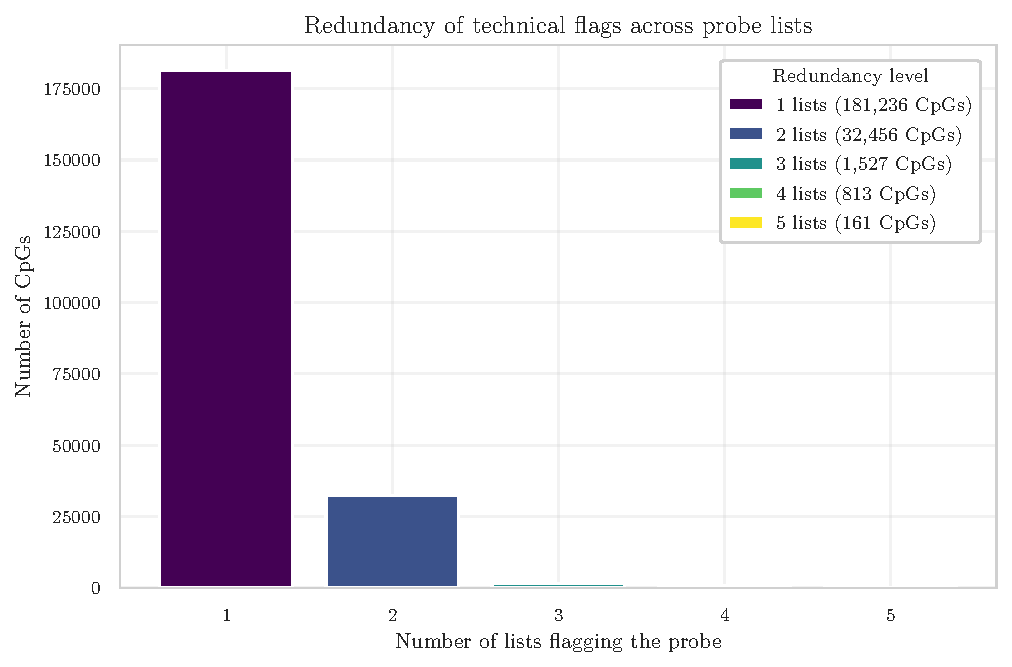
\includegraphics[width=\textwidth]{images/cap4/GSE287331_technical_lists_redundancy_histogram.pdf}
        \caption{
            Redundancy of probes flagged by 1--5 lists.
        }
        \label{fig:gse287331_tech_redundancy}
    \end{subfigure}
    \caption{
        Summary of technical filtering for the methylation dataset.  
        \textbf{(a)} Number of CpGs intersecting each curated resource.  
        \textbf{(b)} Redundancy analysis capturing concordance across filtering lists.
    }
    \label{fig:gse287331_technical_filtering}
\end{figure}

Technical probe filtering excluded CpG loci affected by unreliable hybridisation, SNP interference, multi-mapping or annotation inconsistencies.
Across the established probe-filtering resources, 124{,}511 CpGs were flagged by Naeem, 8{,}992 by the Pidsley blacklist, 102{,}802 by Zhou’s fields, 1{,}730 by Chen’s cross-reactive probe set, and 3{,}672 by McCartney’s cross-hybridisation catalogue.
The union of these lists removed 203{,}114 unique CpGs, leaving 499{,}804 CpGs prior to annotation-based filtering.


\textbf{Annotation-based filtering (Illumina manifest).}
Using the EPIC v1.0 manifest, probes lacking valid genomic coordinates or targeting
non-CpG contexts were removed.  
This eliminated 500 non-CpG probes, reducing the feature set to
499{,}304 CpGs.

\textbf{Removal of sex-chromosome probes (X/Y).}
Probes mapped to chromosomes~X and~Y were removed to avoid sex-driven confounding.
A total of 12{,}579 CpGs were discarded, resulting in an autosomal
working set of 486{,}725 CpGs.

Across all filters, 216{,}193 unique CpGs were removed from the initial
866{,}552, leaving a final autosomal set of 486{,}725 CpGs.
A probe-level removal summary is provided in 
\href{https://github.com/elisabettaroviera/THESIS/blob/main/05%20-%20CpG%20list/Removed%20CpGs%20per%20Dataset/removed_cpgs_all_filters_summary_gse287331.csv}%
{\texttt{removed\_cpgs\_all\_filters\_summary\_gse287331.csv}}.

\begin{table}[t]
\centering
\caption{CpG filtering summary for the GSE287331 dataset.}
\label{tab:gse287331_cpg_filtering}
\begin{tabular}{c c c c c c c c c}
\hline
Initial CpGs &
Naeem &
Pidsley &
Zhou &
Chen &
McCartney &
Non-CpG &
X/Y &
Final CpGs \\
\hline
866{,}552 &
124{,}511 &
8{,}992 &
102{,}802 &
1{,}730 &
3{,}672 &
500 &
12{,}579 &
486{,}725 \\
\hline
\end{tabular}
\end{table}


\paragraph{Step~3 -- $\beta$ to $M$ Conversion}
\label{par:gse287331_step4}

\begin{figure}[t]
    \centering

    % ---------------- ROW 1: HISTOGRAMS ----------------
    \begin{subfigure}{0.24\textwidth}
        
\includegraphics[width=\textwidth]{images/cap4/GSE287331_hist_normal_beta.pdf}
        \caption{Normal ($\beta$)}
    \end{subfigure}
    \begin{subfigure}{0.24\textwidth}
        
\includegraphics[width=\textwidth]{images/cap4/GSE287331_hist_adjacent_beta.pdf}
        \caption{Adjacent ($\beta$)}
    \end{subfigure}
    \begin{subfigure}{0.24\textwidth}
        
\includegraphics[width=\textwidth]{images/cap4/GSE287331_hist_normal_m.pdf}
        \caption{Normal ($M$)}
    \end{subfigure}
    \begin{subfigure}{0.24\textwidth}
        
\includegraphics[width=\textwidth]{images/cap4/GSE287331_hist_adjacent_m.pdf}
        \caption{Adjacent ($M$)}
    \end{subfigure}

    \vspace{0.35cm}

    % ---------------- ROW 2: MEAN–SD RELATIONS ----------------
    \begin{subfigure}{0.24\textwidth}
        
\includegraphics[width=\textwidth]{images/cap4/GSE287331_msd_normal_beta.pdf}
        \caption{Mean--SD (Normal, $\beta$)}
    \end{subfigure}
    \begin{subfigure}{0.24\textwidth}
        
\includegraphics[width=\textwidth]{images/cap4/GSE287331_msd_adjacent_beta.pdf}
        \caption{Mean--SD (Adjacent, $\beta$)}
    \end{subfigure}
    \begin{subfigure}{0.24\textwidth}
        
\includegraphics[width=\textwidth]{images/cap4/GSE287331_msd_normal_m.pdf}
        \caption{Mean--SD (Normal, $M$)}
    \end{subfigure}
    \begin{subfigure}{0.24\textwidth}
        
\includegraphics[width=\textwidth]{images/cap4/GSE287331_msd_adjacent_m.pdf}
        \caption{Mean--SD (Adjacent, $M$)}
    \end{subfigure}

    \caption{Distributional comparison of $\beta$ and $M$ in Normal and Adjacent
tissues in GSE287331.}
    \label{fig:gse287331_beta_m_combined}
\end{figure}


Given the strong mean--variance dependence intrinsic to $\beta$-values, the working
matrix obtained after technical and invariance filtering  
(486{,}725 CpGs across 311 samples) 
was transformed into $M$-values.
This transformation yields an approximately homoscedastic scale and is the standard
input for linear models, empirical Bayes moderation, and batch-effect correction.

The transformation was applied to all CpG columns (284{,}745 CpGs, excluding
\texttt{id\_tissue} and \texttt{label}).  
The resulting object, \texttt{M\_clean}, preserves the same schema as the
$\beta$-matrix and was stored as a memory-efficient \texttt{LazyFrame}.

\textbf{Distributional effects of the $\beta \rightarrow M$ transformation.}
Figure  \ref{fig:gse287331_beta_m_combined} illustrates the
impact of the transformation on the empirical data distribution.  
As expected, the U-shaped $\beta$-profiles for Normal and Adjacent tissues become
substantially more symmetric after conversion, while the pronounced mean--SD
dependence flattens into a markedly more stable variance structure across the full
range of $M$-values.  
These properties make $M$-values preferable for statistical modelling, whereas
$\beta$-values are retained for biological interpretation and visualisation.


% ============================================================


\section{Cross-Dataset Effects of Preprocessing}
\label{sec:inter_preprocessing}

After completing the intra-dataset pre-processing for each cohort, a concise inter-dataset analysis is performed to summarise the effects of the pipeline and to motivate the subsequent feature selection step. 
\paragraph{Pverview of the pre-processing pipeline}
All three datasets underwent a harmonised pre-processing workflow, including initial integrity checks, literature-based technical filtering, manifest-driven probe validation, removal of sex-chromosome loci, and transformation from $\beta$-values to M-values. While the specific implementation details differ slightly depending on platform characteristics and data quality, the conceptual structure of the pipeline is consistent across datasets.

Table~\ref{tab:preprocessing-summary} reports, for each dataset, the number of samples retained and the dimensionality of the methylation matrix before and after pre-processing. Despite substantial differences in initial platform coverage (450K vs EPIC), technical filtering consistently removes a large fraction of probes, yielding cleaner and more reliable feature spaces.

\begin{table}[t]
\centering
\caption{Summary of sample size and CpG dimensionality before and after pre-processing.}
\label{tab:preprocessing-summary}
\begin{tabular}{lcccccc}
\hline
Dataset & Platform & Normal & Adjacent & CpGs \textit{before} pre-processing & CpGs \textit{after} pre-processing \\
\hline
GSE69914  & 450K  & 50  & 42  & 485{,}512 & 251{,}483 \\
GSE225845 & EPIC & 113 & 140 & 750{,}426 & 530{,}683 \\
GSE287331 & EPIC & 182 & 60  & 866{,}554 & 486{,}725 \\
\hline
\end{tabular}
\end{table}

\paragraph{CpG overlap across datasets}
To further characterise the relationship between datasets, CpG overlap was evaluated both before and after pre-processing. Figure~\ref{fig:venn-pre} illustrates the overlap of CpG identifiers across the three datasets prior to filtering, reflecting platform design constraints and baseline annotation differences. As expected, the intersection is dominated by probes shared between the two EPIC datasets, with a smaller but substantial core common to all three cohorts.

Figure~\ref{fig:venn-post} reports the corresponding overlap after the complete pre-processing pipeline. Although the total number of CpGs is markedly reduced, a large shared core remains, indicating that technical filtering primarily removes platform- or annotation-specific probes while preserving a common, high-confidence CpG backbone.

\begin{figure}[t]
\centering
\begin{subfigure}[t]{0.48\textwidth}
    \centering
    
\includegraphics[width=\textwidth]{images/cap4/venn_cpg_overlap_pre_preprocessing.pdf}
    \caption{CpG overlap across datasets before pre-processing.}
    \label{fig:venn-pre}
\end{subfigure}
\hfill
\begin{subfigure}[t]{0.48\textwidth}
    \centering
    
\includegraphics[width=\textwidth]{images/cap4/venn_cpg_overlap_post_preprocessing.pdf}
    \caption{CpG overlap across datasets after pre-processing.}
    \label{fig:venn-post}
\end{subfigure}
\caption{Comparison of CpG overlap across datasets before and after pre-processing.}
\label{fig:venn-comparison}
\end{figure}


\section{Post-Preprocessing Data Structure and Feature Selection Rationale}
Despite extensive technical filtering, the post-processed datasets remain highly dimensional, with hundreds of thousands of CpGs retained in each cohort. Moreover, the large shared CpG intersection across datasets suggests that technical artefacts have been effectively mitigated, shifting the primary challenge from data quality to signal extraction.

At this stage, the limiting factor is no longer technical reliability but statistical and biological relevance. The remaining feature space is expected to contain a substantial proportion of CpGs that are either weakly informative or irrelevant for distinguishing Normal and Adjacent breast tissue. Consequently, a dedicated feature selection strategy is required to identify a reduced subset of CpGs that captures biologically meaningful variation while improving interpretability, robustness, and downstream modelling performance.

The next chapter therefore focuses on feature selection methodologies applied to these pre-processed datasets, building on the stable and harmonised CpG space established here.


